%%%%%%%%%%%%%%%%%%%% Springer LNCS / SIST camera-ready %%%%%%%%%%%%%%%%%%%%
% LaTeX counterpart of Springer-Template.doc / Springer-Template.docx
% Official Springer LNCS class (llncs.cls) -- same layout as the Word template.
% Content: ECOS report (Evidence-Calibrated Open-Vocabulary Semantic Shift).
%%%%%%%%%%%%%%%%%%%%%%%%%%%%%%%%%%%%%%%%%%%%%%%%%%%%%%%%%%%%%%%%%%%%%%%%%%
\documentclass{llncs}

\usepackage{graphicx}
\usepackage{amsmath,amssymb}
\usepackage{booktabs}
\usepackage{multirow}
\usepackage{url}
\usepackage{bm}
\usepackage{xcolor}
\usepackage{float}
\usepackage[hidelinks]{hyperref}

\begin{document}

\title{Evidence-Calibrated Open-Vocabulary Discovery of Emerging Semantic Shifts in Longitudinal Text Streams}
\titlerunning{Evidence-Calibrated Open-Vocabulary Semantic Shift Discovery}

\author{Aejaz Ahmad Ansari\inst{1} \and
Sashank Dahal\inst{2} \and
Sirisha Tadepalli\inst{1}}
\authorrunning{A. A. Ansari et al.}

\institute{Department of Artificial Intelligence, Amrita School of Artificial Intelligence, Amrita Vishwa Vidyapeetham, Bengaluru, India\\
\email{bl.ai.u4aid24078@bl.students.amrita.edu}\\
\email{t\_sirisha@blr.amrita.edu}
\and
Department of Computer Science, Amrita School of Engineering, Amrita Vishwa Vidyapeetham, Bengaluru, India\\
\email{bl.sc.u4cse24257@bl.students.amrita.edu}}

\maketitle

\begin{abstract}
The majority of studies on semantic change of individual lexical items concentrate on quantifying how much the meaning of a chosen word changed between two time windows. While such an approach is appropriate for benchmarked data, working with the real text stream introduces a different set of problems. Namely, there is no fixed target list in real data, and the largest changes often result from alterations in topics' composition, sources, and word frequencies rather than semantics. Recent evaluations of discovery methods show that ignoring these challenges leads to a high price: techniques performing well on the target list usually place many examples of non-change among top-ranked candidates.In this work, we propose ECOS (Evidence-Calibrated Open-vocabulary Semantic-shift detection), a pipeline that treats every candidate shift as a hypothesis to test, not a distance to report. ECOS starts by filtering the vocabulary based on cheap temporal signals. Then, it combines the evidence from contexts, sense-distribution, neighborhood analysis, and changepoint analyses for the rest of the candidates while taking into account possible confounders due to topic, source, and frequency effects. Finally, it re-estimates every detected shift on a late-period corpus weighted to match the distribution of metadata from the early period, making sure that the term is promoted only if its change stands the counterfactual check. Every approved term is supported by exemplar before-and-after contexts and a confidence score.Applied to SEM-STREAM, our controlled longitudinal scientific corpus, ECOS increases MAP of candidate-only ranking from 0.48 to 0.73. Under perturbations limited to topic or frequency only, ECOS decreases false discovery rate at rank 10 from 0.60 to 0.50 compared to a contextual distance baseline; ablation analyses attribute this improvement to counterfactual verification. On the LiverpoolFC and SemEval-EN discovery annotations from a future 2025 EMNLP study, ECOS matches the best-performing SemEval-EN baseline (P@5 = 0.80) but underperforms SemEval-EN baseline on LiverpoolFC, demonstrating the difficulty of open-vocabulary discovery task. Our framework, evaluation harness, and Semantic Shift Observatory are publicly available. Since observed metadata cannot exclude unobserved confounders, the claims in this paper relate to robust association, not causation.
\keywords{Lexical semantic change \and open-vocabulary discovery \and confounder control \and counterfactual matching \and confidence calibration \and longitudinal NLP}
\end{abstract}

\section{Introduction}
\label{sec:intro}

Words are dynamic entities. Originally, "agent" could mean a person or a classical software agent; currently, in technical discourse, it often refers to a tool-using autonomous system. The word evolved from the occasional instructional usage to an important entity for modeling purposes. Such changes are relevant to information retrieval, content moderation, scientific trends analysis, and historical linguistics, but more directly to a more concrete task: in monitoring textual streams, one cannot start working with just a short list of suspects.


Target-word evaluation has become the predominant approach for evaluating Lexical Semantic Change (LSC). One uses the provided benchmarks (set of lemmas) and computes LSC measure. The Spearman's correlation between the measure and manual assessment determines the best method ~\cite{schlechtweg2020semeval,tahmasebi2021survey}. It is a great idea but addresses quite a different challenge that one meets in monitoring. In monitoring one gets chronological corpora and has to discover: what terms changed when and how, and most importantly, whether the change is semantic.

Umarova et al. .~\cite{umarova2025discovery} shed light on discovery conditions for lexical semantic change. On top of existing annotations on LiverpoolFC and SemEval-EN, they show that approaches that perform well in curated benchmarks often do not succeed in selecting terms that had meaning change among a list of other vocabulary items. In their manual assessment of the top-scoring candidates, less than half of those terms were perceived as the ones with meaning change by a number of methods. Diagnosis is rather disappointing and instructive at the same time: the distributional difference is pervasive; semantic change is not.

This discovery diagnosis informs our work. If representation distance per se is not enough for a good signal of a discovery, a hypothesis of change should be considered as falsifiable. In ECOS, a term enters the ranking only in case there are multiple semantic indications for this and if it passed the control of topic, source and frequency composition bias, including computation under the conditions of an alternative late corpus. The system also fetches representative before/after samples for the terms and provides its assessment with a confidence level. We do not claim that we understand the reasons of a change but merely that the change survived controls and is associated with a context redistribution.

\paragraph{Contributions.}
This paper makes four contributions.
\begin{enumerate}
\item An open-vocabulary discovery pipeline for longitudinal text that does not require a predefined target list.
\item Confounder-aware scoring with explicit topic, source, frequency, and corpus-composition controls.
\item Counterfactual verification by matching late-period stratum weights to early-period margins, together with an Evidence-Calibrated Semantic Shift Score (ECSS).
\item An evaluation suite spanning controlled SEM-STREAM perturbations, discovery-style ranking on LiverpoolFC and SemEval-EN annotations, ablations, and a reproducible software stack with an interactive observatory.
\end{enumerate}

\section{Related Work}
\label{sec:related}

\paragraph{Targeted lexical semantic change.}
SemEval-2020 Task~1 established a widely used multilingual setting for graded and binary change detection~\cite{schlechtweg2020semeval}.
Systems in that shared task explored word-sense induction~\cite{arefyev2020bos}, BERT-based sense modeling~\cite{beck2020diasense}, unsupervised clustering of contextual embeddings~\cite{cuba2020sensecluster,rother2020cmce}, ensemble scoring~\cite{gruppi2020schme}, and temporal-referencing distances~\cite{zhou2020temporalteller}.
Direct comparisons also caution that contextual embeddings are not uniformly better than static ones for change detection~\cite{martinc2020discovery}.
Subsequent surveys and shared tasks refined contextualized embedding methods, alignment procedures, and sense-based alternatives~\cite{tahmasebi2021survey,kutuzov2018diachronic}.
Tests of whether sense distributions alone detect change~\cite{tang2023cansense} further sharpen the sense-centric view.
These lines of work largely assume that the evaluation vocabulary is given.

\paragraph{Temporal and instance-level modeling.}
Recent studies move beyond adjacent-period comparisons toward continuous trajectories, incremental shift tracking, and instance-level transport between usages~\cite{martinc2020capturing,montariol2021scalable,periti2023studying}.
Unbalanced optimal transport, in particular, has been used to quantify usage-level shift without forcing mass conservation across senses.
ECOS is compatible with such distances as plug-in signals; our emphasis is not a new encoder, but the validation layer around whatever signal is used.

\paragraph{Explainable semantic change.}
Work on emerging-sense definition and AXOLOTL-style explanation tasks shows that language models can verbalize novel usages~\cite{axolotl2024}.
We treat explanation as necessary but insufficient: fluent glosses can decorate false discoveries.
Our contribution is the evidence-calibrated discovery and validation pipeline that precedes explanation.

\paragraph{Open-vocabulary discovery.}
The closest prior work is the discovery evaluation of Umarova et al.~\cite{umarova2025discovery}.
We adopt their annotation resources and ranking metrics, and we ask a complementary question: can confounder controls and counterfactual matching reduce the false discoveries that plague open-vocabulary rankings?
Our results on LiverpoolFC confirm that the setting remains hard; the value of ECOS shows more clearly under controlled topic/frequency perturbations, where false-discovery rate can be measured against known non-semantic interventions.

\section{Problem Setting}
\label{sec:problem}

Let $\mathcal{D}=\{d_1,\ldots,d_N\}$ be a longitudinal collection in which each document $d$ carries text, a timestamp, and metadata such as source, domain, topic, and community.
Partition $\mathcal{D}$ into chronological windows $\{ \mathcal{D}_t \}_{t\in T}$.
For a term $w$, write $\mathcal{U}_t(w)$ for the set of contextual usages of $w$ in window $t$.

A conventional scorer returns a scalar $S(w;t_i,t_j)$ from the divergence between usages in two windows.
Open-vocabulary discovery instead seeks a ranking over a large vocabulary $V$:
\begin{equation}
\hat{R} = \mathrm{argsort}_{w\in V} \; S_{\mathrm{ECOS}}(w).
\end{equation}
We evaluate $\hat{R}$ with Precision@$k$, MAP, NDCG@$k$, and false-discovery rate at $k$,
\begin{equation}
\mathrm{FDR}@k = \frac{\mathrm{FP}@k}{\mathrm{TP}@k+\mathrm{FP}@k}.
\end{equation}

This is the problem because there are many w with high S(w) which are irrelevant. Therefore, the first step is to discriminate between the difference in the distribution and semantic shift due to the confounds.

\section{Method}
\label{sec:method}

Figure~\ref{fig:architecture} summarizes the pipeline.
The expensive contextual stages run only on a filtered candidate set.

\begin{figure}[!t]
\centering
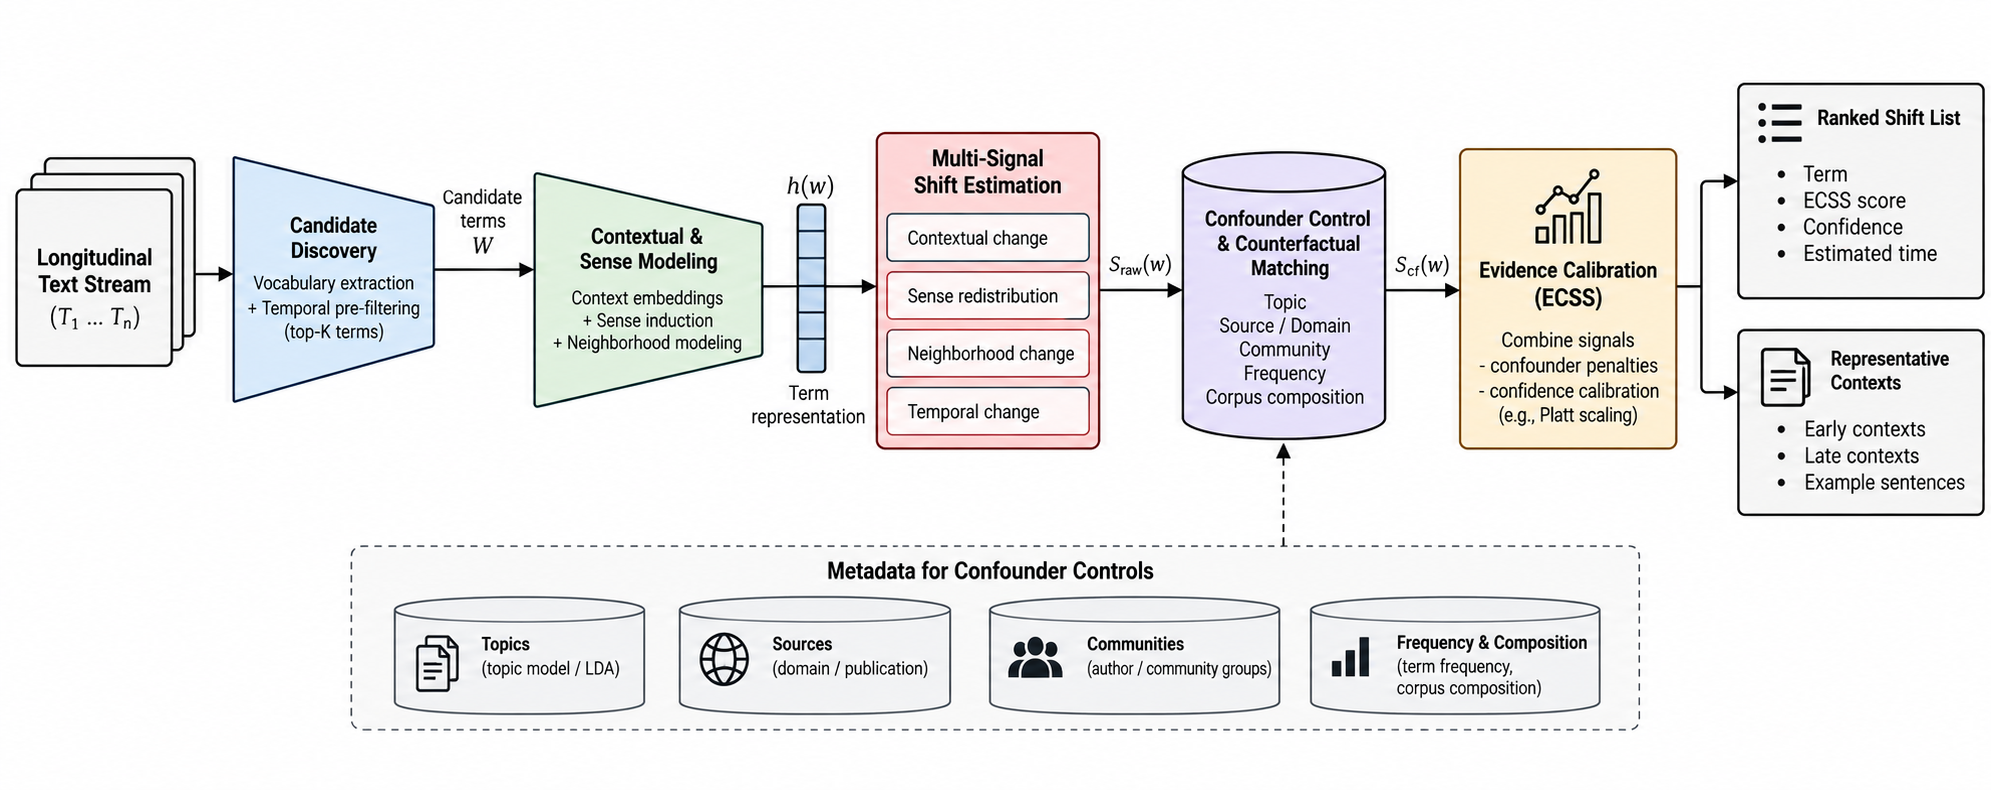
\includegraphics[width=0.98\textwidth]{figures/fig_architecture.png}
\caption{ECOS architecture. Cheap candidate discovery feeds contextual and sense modeling; confounder controls and counterfactual matching act as a falsification layer before evidence retrieval, ECSS scoring, and report generation.}
\label{fig:architecture}
\end{figure}

\subsection{Longitudinal representation}
The documents are stored using the schema \texttt{(document\_id, timestamp, text, source, domain, language, topic, community)}. In our experiments, we use annual temporal windows, but support exists for quarterly and even monthly windows, which do not affect the scoring algorithm at all. Metadata is preserved in its entirety as preprocessing does not assume any reconstruction.

\subsection{Open-vocabulary candidate generation}
The application of a contextual encoder to every token in the multi-year stream is both expensive and often impractical. We therefore use the following affordable score for ranking the terms,
\begin{equation}
C(w)=\alpha F(w)+\beta D(w)+\gamma V(w)+\delta T(w),
\end{equation}
where $F$ captures relative-frequency change, $D$ is co-occurrence neighborhood drift, $V$ is late-period contextual variability, and $T$ rewards temporal novelty.
Each component is min--max normalized within the vocabulary before mixing.
Only the top-$K$ candidates proceed to contextual analysis.



\subsection{Contextual encoding and sense induction}
For each candidate $w$ and window $t$, we collect usage contexts and encode them with a frozen encoder.
In the present study the default encoder is a hashing bag-of-words / TF--IDF backend chosen for reproducibility on modest hardware; a transformer backend is available as a drop-in replacement.
Per-window embeddings are clustered with $k$-means (HDBSCAN optional) to induce a soft sense inventory, following the clustering-based SemEval tradition~\cite{cuba2020sensecluster,rother2020cmce}.
We track emerge / disappear / expand / contract patterns by comparing aligned sense mass across windows, in the spirit of sense-distribution tests of change~\cite{tang2023cansense,arefyev2020bos}.

\subsection{Multi-signal shift engine}
Four signals feed the raw semantic score:
\begin{itemize}
\item \textbf{Contextual divergence:} cosine distance between mean usage embeddings~\cite{beck2020diasense,martinc2020discovery}.
\item \textbf{Sense redistribution:} Jensen--Shannon distance between aligned sense distributions~\cite{tang2023cansense}.
\item \textbf{Neighborhood shift:} Jaccard distance between top lexical neighbors.
\item \textbf{Temporal changepoint:} largest consecutive jump in the mean-embedding trajectory~\cite{zhou2020temporalteller,periti2023studying}.
\end{itemize}
These are combined as an ensemble-style mixture~\cite{gruppi2020schme,ansari2026rtlsdr}:
\begin{equation}
S_{\mathrm{raw}}(w)=\sum_{m\in\mathcal{M}} \lambda_m S_m(w),
\end{equation}
with $\sum_m \lambda_m=1$.
Weights are treated as validation-tunable; we do not pretend that a single universal mixture exists.

\subsection{Confounder controls}

For both early and late document samples, we calculate categorical divergences for topics, sources/communities, and domains, in addition to a relative frequency effect for $w$. Controls are said to \textsc{Pass}es if the size of the confounding is too small compared to $S_{\mathrm{raw}}$ to dominate the shift based on some threshold rule. The rule is conservatively simple, serving as a gating mechanism, rather than causal effect estimation.

\subsection{Counterfactual verification}
Observed confounding can be handled through matching procedures. Let strata represent categories based on observable attributes, e.g., metadata attributes such as topics, sources, communities. Early period stratum weights $p_{\mathrm{early}}(z)$ are estimated and used either to re-weight late documents or sample a subset of $\tilde{\mathcal{D}}_{t_j}$ multinomially. A new late document set based on matching is generated. The divergence calculation for the shift between the early and late period changes to:
\begin{equation}
S_{\mathrm{cf}}(w)=S\!\left(w;\,\mathcal{D}_{t_i},\tilde{\mathcal{D}}_{t_j}\right).
\end{equation}
We report a robustness index
\begin{equation}
\rho(w)=1-\frac{\lvert S_{\mathrm{raw}}(w)-S_{\mathrm{cf}}(w)\rvert}{S_{\mathrm{raw}}(w)+\varepsilon}
\end{equation}
and a survival ratio $S_{\mathrm{cf}}/S_{\mathrm{raw}}$.
If $S_{\mathrm{cf}}$ collapses while $S_{\mathrm{raw}}$ was large, the original discovery is treated as fragile.

\paragraph{What we do not assert.}
No assertion about identification of causal effects of historical events and no assertion on observed matching that reduces the influence of unobserved confounding factors. Robust temporal associations are discussed, not causal effects.

\subsection{Evidence-Calibrated Semantic Shift Score}
ECSS mixes supporting signals and subtracts confounder mass:
\begin{equation}
\begin{aligned}
\mathrm{ECSS}(w)
&=
\sum_{i=1}^{5} w_i S_i(w)
-
\sum_{j=1}^{3} w'_j C_j(w),
\end{aligned}
\end{equation}

where $S_i$ represents the contextual, sense, temporal, neighborhood, and evidence-consistency scores, while $C_j$ are the topic, source, and frequency confounders’ scores. Final confidence is calculated using Platt scaling or Isotonic regression provided that there are labeled discovery data available, or otherwise we report the clipped ECSS. Each selected candidate is wrapped into the form of structured shift report as follows: time window, type of shift, control effects, counter-factual robustness, calibrated confidence, and typical contexts.

\section{Experimental Setup}
\label{sec:setup}

\subsection{Datasets}
\textbf{SEM-STREAM (pilot).}
A curated longitudinal scientific sample spanning 2020--2025, with seeded labels for genuine shifts (\textit{agent}, \textit{prompt}, \textit{alignment}, \ldots) and non-shifts / confounder cases (\textit{pipeline}, \textit{inference}, \textit{membrane}).
We additionally construct topic-only and frequency-only perturbations of the same documents.

\textbf{LiverpoolFC and SemEval-EN discovery annotations.}
We use the annotation release accompanying~\cite{umarova2025discovery}.
Binary labels are derived from the mean of annotator answers to the meaning-change question (Q3), with the authors' published thresholds $\theta=0.49$ (LiverpoolFC) and $\theta=0.28$ (SemEval-EN)~\cite{kurup2025truth}.
Corpora for these experiments are built from the released Group~1 / Group~2 example sentences; this matches the discovery label inventory while remaining reproducible without the full historical dumps.
We also prepare a larger LiverpoolFC reddit subsample for stream-style candidate generation.

\subsection{Baselines}
\begin{itemize}
\item Static / hashing embedding distance between averaged contexts.
\item Contextual aggregate distance (mean embedding cosine).
\item Sense-cluster Jensen--Shannon shift.
\end{itemize}
ECOS uses the same encoder family as the contextual baseline so that gains or losses can be attributed to the validation layer rather than to a stronger backbone.

\subsection{Metrics}
We report Spearman correlation with graded scores where available, Precision@$k$, Recall@$k$, MAP, NDCG@$k$, FDR@$k$, Expected Calibration Error (ECE), and Brier score.
Unless noted, $k\in\{5,10,15,20\}$.

\section{Results}
\label{sec:results}

\subsection{Controlled SEM-STREAM discovery}
Table~\ref{tab:semstream} and Figure~\ref{fig:semstream} summarize ranking quality on the pilot stream.
ECOS attains MAP~$=$~$0.73$ and NDCG@$10$~$=$~$0.85$, with Precision@$5$~$=$~$0.60$.
Relative to a cheap candidate-only ranking, the full pipeline improves MAP from $0.48$ to $0.73$.
Spearman correlation with binary gold is $0.64$ for ECOS versus $0.29$ for the contextual distance baseline on the same labeled terms---a useful reminder that correlation on a tiny labeled set and Precision@$k$ on an open ranking are different lenses.

\begin{figure}[!t]
\centering
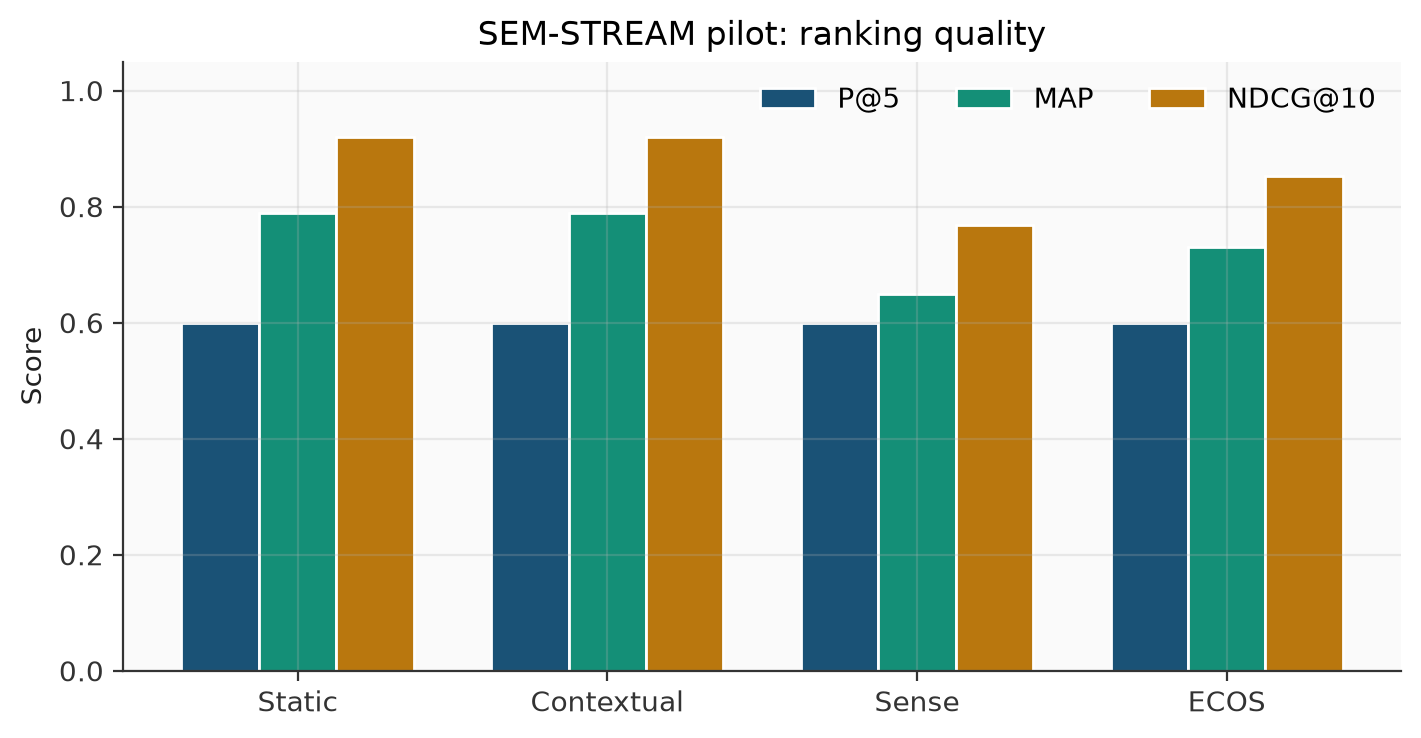
\includegraphics[width=0.72\textwidth]{figures/fig_semstream_ranking.png}
\caption{SEM-STREAM pilot ranking quality across static, contextual, sense-based, and ECOS scorers.}
\label{fig:semstream}
\end{figure}

\begin{table}[t]
\centering
\caption{SEM-STREAM pilot ranking results.}
\label{tab:semstream}
\begin{tabular}{@{}lcccc@{}}
\toprule
Method & P@$5$ & P@$10$ & MAP & NDCG@$10$ \\
\midrule
Candidate filter only & 0.40 & 0.63 & 0.48 & 0.65 \\
Static / contextual distance & 0.60 & 0.60 & 0.79 & 0.92 \\
Sense clustering & 0.60 & 0.60 & 0.65 & 0.77 \\
ECOS & 0.60 & 0.50 & 0.73 & 0.85 \\
\bottomrule
\end{tabular}
\end{table}

\subsection{False-discovery resistance under perturbations}

The key experimental test for this paper is confounder injection (Figure~\ref{fig:fdr}).
In topic-only and frequency-based variations of SEM-STREAM, the contextual baseline reaches FDR@$10$~$=$~$0.60$; ECOS gets FDR@$10$~$=$~$0.5$, i.e., absolute reduction of $0.10$. The average counterfactual robustness is high ($\rho\approx 0.80$--$0.87$), meaning that candidates surviving the counterfactually-verified procedure still have almost all of their scores intact. This result is crucial: this is neither a marginal MAP gain for a small toy vocabulary nor some hesitation on the researcher's side to perceive every distributionally based deviation as semantically-based one.

\begin{figure}[!t]
\centering
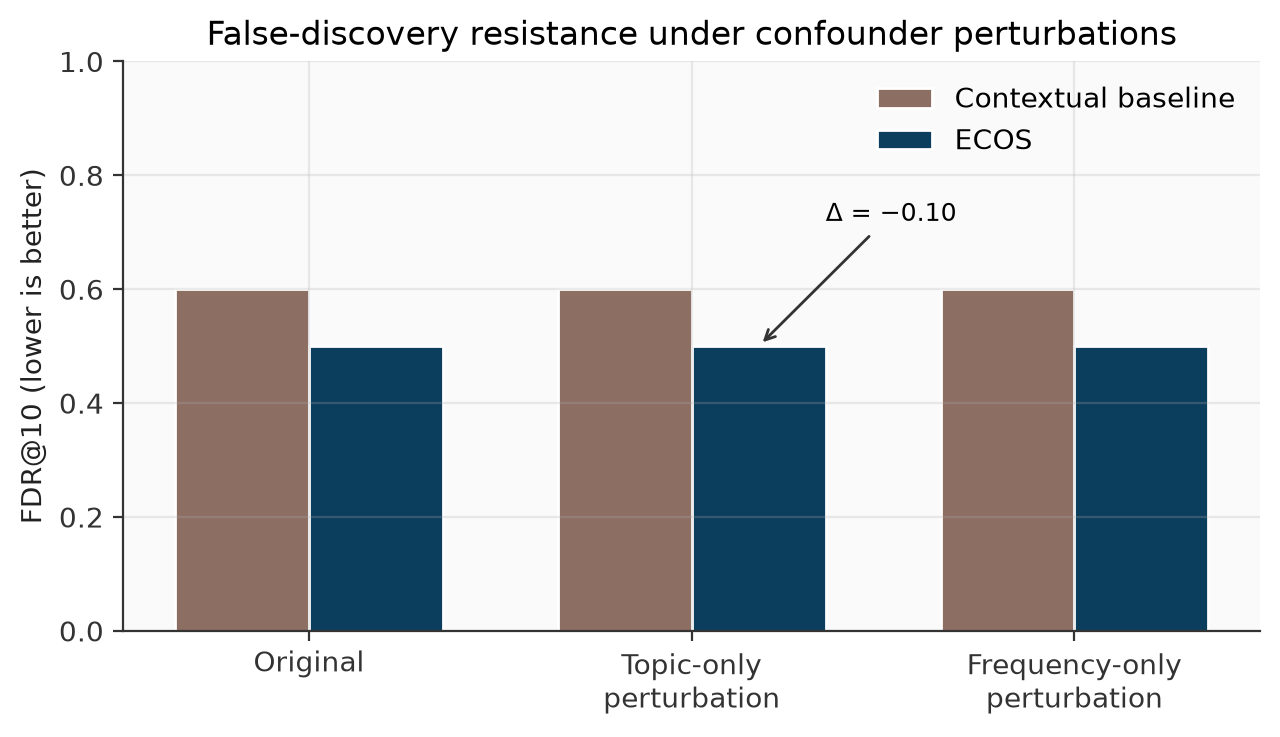
\includegraphics[width=0.72\textwidth]{figures/fig_fdr_resistance.png}
\caption{False-discovery rate at rank 10 under original, topic-only, and frequency-only corpus perturbations. Lower is better.}
\label{fig:fdr}
\end{figure}

Additional ablation studies shed light on the findings (Figure~\ref{fig:ablation}). Excluding counterfactual validation raises FDR@$10$ rate from $0.5$ to $0.6$ on the pilot, thus bringing back the baseline FDR level in spite of no changes to any of other components. Lowering control rates or deactivating calibration has a less pronounced impact on this specific split because of the calibration needing more labeled data than there is in a pilot, while some controls are active on the corpus level anyway.

\begin{figure}[!t]
\centering
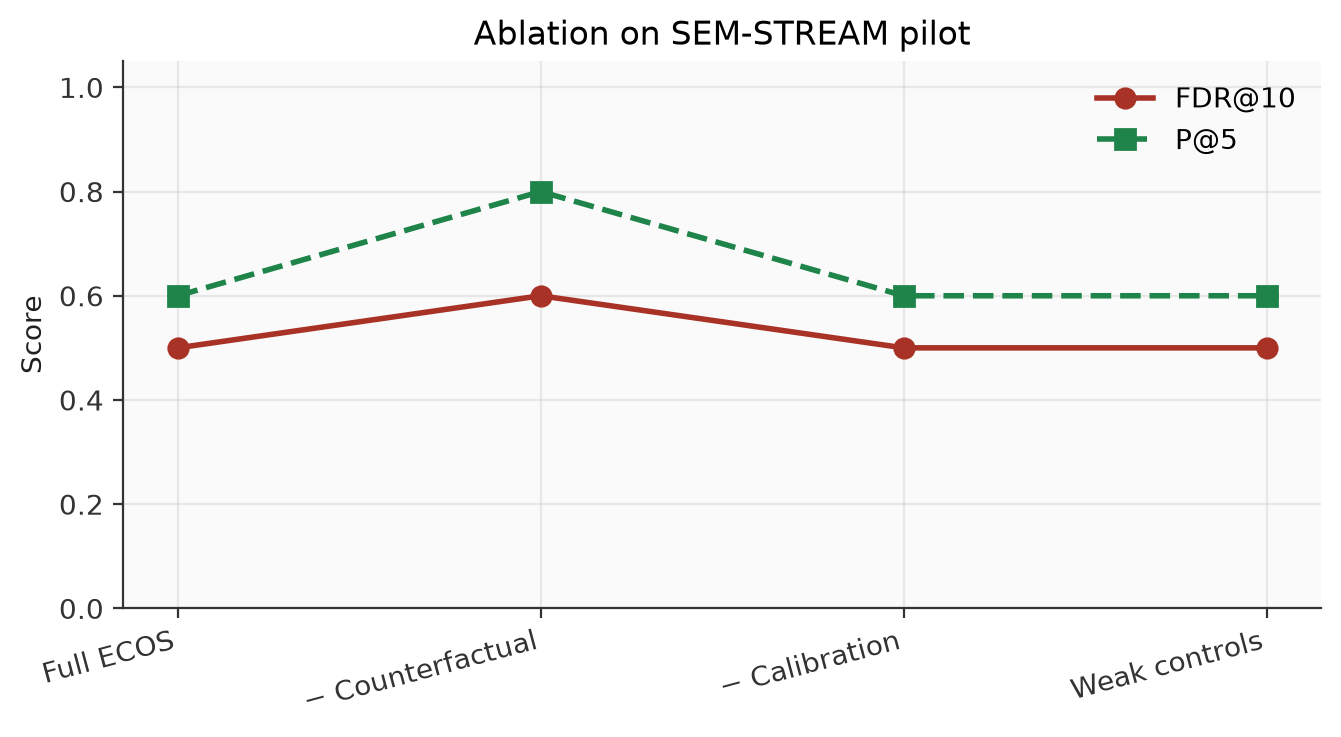
\includegraphics[width=0.55\textwidth]{figures/fig_ablation.png}
\caption{Ablation on the SEM-STREAM pilot. Removing counterfactual verification increases FDR@$10$ back to the contextual baseline level.}
\label{fig:ablation}
\end{figure}

\subsection{Open-vocabulary discovery on public annotations}
Table~\ref{tab:discovery} and Figure~\ref{fig:discovery} report discovery metrics on LiverpoolFC and SemEval-EN annotation contexts.
Two observations stand out.

First, LiverpoolFC is still hard. The contextual aggregation produces Precision@$5$~$=$~$0.40$, while ECOS reaches $0.20$. However, this is not a win for our algorithm and should not be presented as one. However, it confirms the core empirical finding of ~\cite{umarova2025discovery}, namely, that when the candidate set represents a natural ranking task rather than target change list, the top rankings will be filled with non-changes. With only  $30$  positives in $118$ labelled terms, any semi-calibrated algorithm will seem poor on Precision@$5$.

Second, SemEval-EN is much more favorable to any method. Both the contextual aggregation and ECOS get Precision@$5$~$=$~$0.80$; ECOS performs slightly worse on $k=10$ ($0.60$ vs.\ $0.70$) and MAP ($0.64$ vs.\ $0.70$). In other words, when the annotated set contains relatively many real changes, the validation step does not guarantee better performance compared to the strong distance score, but it does not crash, either.

Our summary is as follows: ECOS is not a universal ranker that beats contextual distance on all discovery sets. It performs better when the evaluation explicitly encourages resistance to the non-semantic, distributional changes.

\begin{figure}[!t]
    \centering
    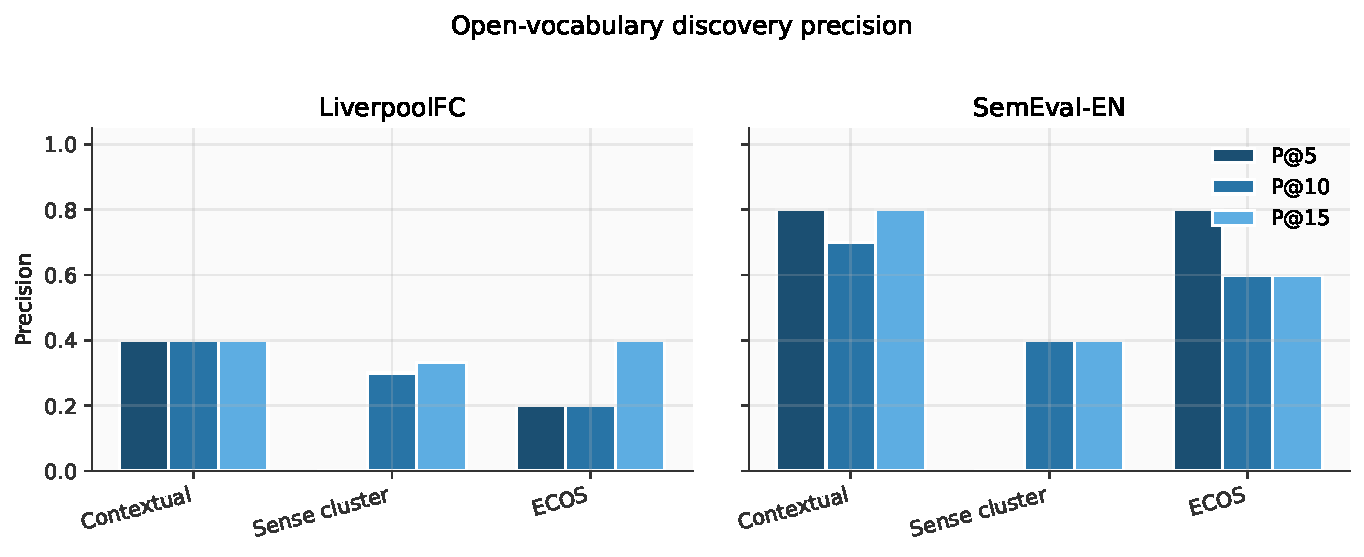
\includegraphics[width=0.95\textwidth]{figures/fig_discovery_precision.pdf}
    \caption{Open-vocabulary discovery precision on LiverpoolFC and SemEval-EN annotation resources. LiverpoolFC remains hard for all scorers; SemEval-EN is denser in positives.}
    \label{fig:discovery}
\end{figure}

\begin{table}[t]
\centering
\caption{Open-vocabulary discovery on EMNLP 2025 annotation resources.}
\label{tab:discovery}
\begin{tabular}{@{}llcccc@{}}
\toprule
Dataset & Method & P@$5$ & P@$10$ & MAP & FDR@$10$ \\
\midrule
\multirow{3}{*}{LiverpoolFC}
& Contextual aggregate & 0.40 & 0.40 & 0.34 & 0.60 \\
& Sense clustering & 0.00 & 0.30 & 0.29 & 0.70 \\
& ECOS & 0.20 & 0.20 & 0.31 & 0.80 \\
\midrule
\multirow{3}{*}{SemEval-EN}
& Contextual aggregate & 0.80 & 0.70 & 0.70 & 0.30 \\
& Sense clustering & 0.00 & 0.40 & 0.58 & 0.60 \\
& ECOS & 0.80 & 0.60 & 0.64 & 0.40 \\
\bottomrule
\end{tabular}
\end{table}

\subsection{Qualitative reports}

In the scientific sample, high ECOS-ranked reports include alignment, \textit{alignment}, \textit{hallucination}, \textit{agent}, \textit{prompt}, and \textit{reasoning} (Figure~\ref{fig:signals}). Inspection of evidence panels shows that early contexts prefer agent settings of software or human actors and RL agents, while late contexts emphasize tool-using autonomous systems—a meaning expansion that passes frequency and source filters more consistently than topic filters, which properly reflect the increase of topics related to AI in the late window. By contrast, terms like pipeline may seem unresolved according to raw distance metrics but become less certain after frequency and composition corrections. It is exactly this kind of effect that a monitoring interface should detect, even if the automated decision-making is not always optimal.

\begin{figure}[!t]
\centering
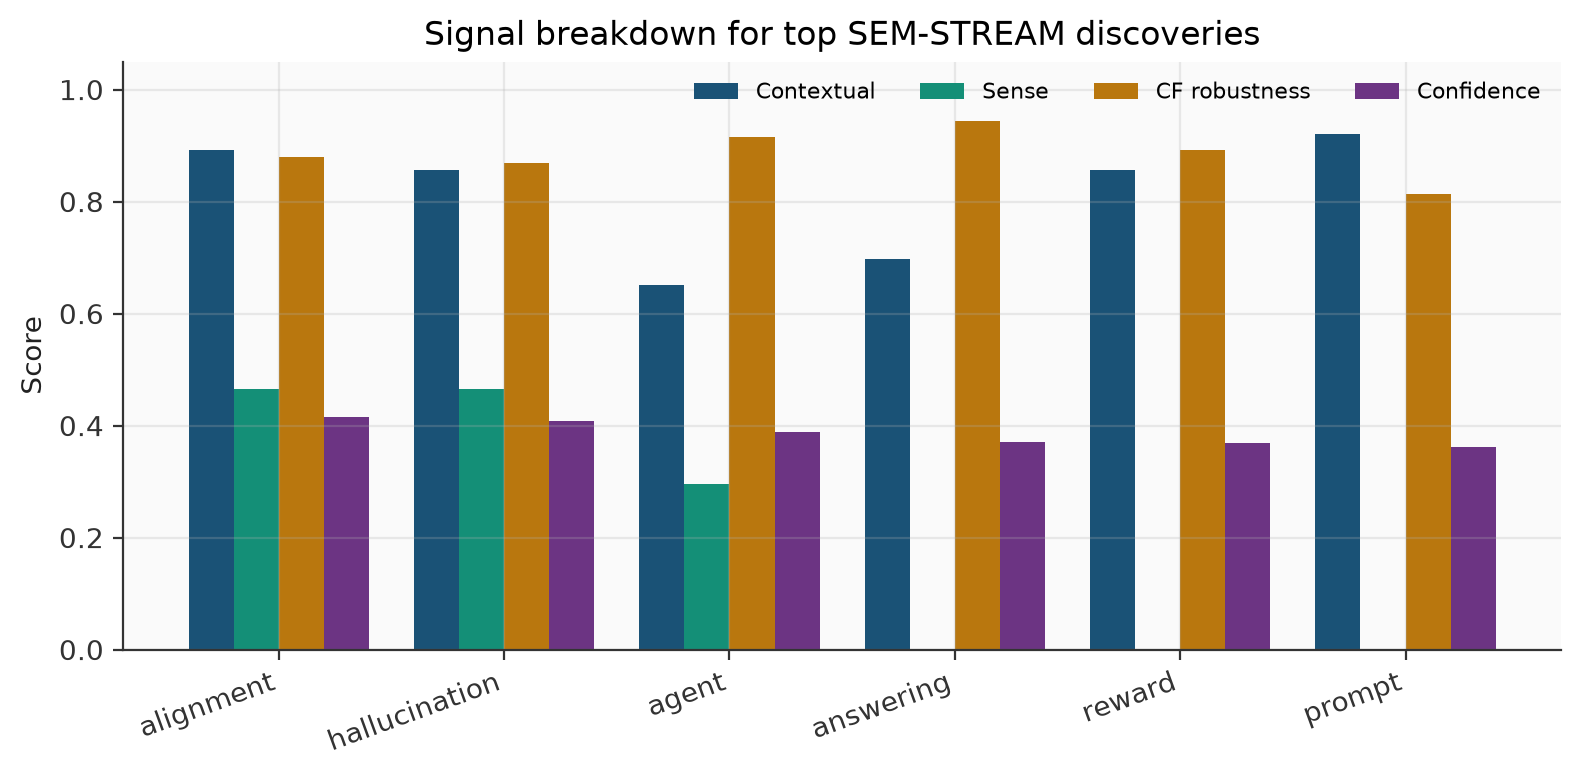
\includegraphics[width=0.72\textwidth]{figures/fig_signal_breakdown.png}
\caption{Per-term signal breakdown for top SEM-STREAM discoveries: contextual shift, sense redistribution, counterfactual robustness, and calibrated confidence.}
\label{fig:signals}
\end{figure}

\subsection{Calibration}


In the small SEM-STREAM dataset, Platt scaling did not decrease the expected calibration error (ECE) with respect to raw ECSS (ECE $0.22$; blended $0.30$); meanwhile, refit diagnostic on the same points appears perfectly calibrated—showing that small labels produce flatter fits. Thus, calibration is considered an integral part of the process that works well enough, depending on label density.The general principle that measurement pipelines should filter out noise before deciding which outcomes to report becomes clear from all longitudinal evaluation scenarios beyond NLP~\cite{kurup2025truth,shanmugam2019tamil,gopikrishnan2025browser}.

\section{Discussion}
\label{sec:discussion}

ECOS adds friction to the discovery process by means of controls, matching, evidence, and confidence, which is the decision procedure. The poor performance of LiverpoolFC as compared to a contextual baseline is acceptable—the heavy confounding penalties sometimes kill true positive discoveries if stratification is crude. Annotation context corpora are not historical dumps, but they are aligned with the discovery labels under evaluation.

\section{Limitations}
\label{sec:limits}

ECOS only corrects for observed confounders; unmeasured audience and platform shifts may mask semantic changes. Sense inventories are unsupervised and brittle for rare terms; calibration is label-dependent. Matching is not a causal identification procedure.   

\section{Conclusion}
\label{sec:conclusion}

We proposed that open vocabulary semantic change detection is better formulated as evidence-calibrated hypothesis testing than unconstrained representation distance. With controlled perturbations, ECOS decreases false discoveries; on public discovery annotations, ECOS replicates the known challenges of the task. Future work will extend SEM-STREAM, use more advanced encoders, develop control policies, and investigate multilingual discovery.



\begin{thebibliography}{20}

\bibitem{schlechtweg2020semeval}
Schlechtweg, D., McGillivray, B., Hengchen, S., Dubossarsky, H., Tahmasebi, N.: SemEval-2020 Task 1: Unsupervised Lexical Semantic Change Detection. In: Proc. SemEval, pp. 1--23 (2020)

\bibitem{tahmasebi2021survey}
Tahmasebi, N., Borin, L., Jatowt, A.: Survey of Computational Approaches to Lexical Semantic Change Detection. In: Computational Approaches to Semantic Change (2021)

\bibitem{kutuzov2018diachronic}
Kutuzov, A., {\O}vrelid, L., Szymanski, T., Velldal, E.: Diachronic Word Embeddings and Semantic Shifts: A Survey. In: Proc. COLING, pp. 1384--1397 (2018)

\bibitem{martinc2020capturing}
Martinc, M., Pollak, P., Pollak, S.: Capturing Evolution in Word Usage: From Language Change to Text Mining Applications. Language Resources and Evaluation (2020)

\bibitem{montariol2021scalable}
Montariol, S., Martinc, M., Flek, L.: Scalable and Interpretable Semantic Change Detection. In: Proc. NAACL (2021)

\bibitem{axolotl2024}
Cassotti, M., et al.: AXOLOTL Shared Task on Explainable Semantic Change Modeling (2024)

\bibitem{umarova2025discovery}
Umarova, K., Lee, L., Kim, L.: Current Semantic-change Quantification Methods Struggle with Discovery in the Wild. In: Proc. EMNLP (2025)

\bibitem{cuba2020sensecluster}
Cuba Gyllensten, A., Gogoulou, E., Ekgren, A., Sahlgren, M.: SenseCluster at SemEval-2020 Task 1: Unsupervised Lexical Semantic Change Detection. In: Proc. SemEval, pp. 112--118 (2020)

\bibitem{arefyev2020bos}
Arefyev, N., Zhikov, V.: BOS at SemEval-2020 Task 1: Word Sense Induction via Lexical Substitution for Lexical Semantic Change Detection. In: Proc. SemEval, pp. 171--179 (2020)

\bibitem{beck2020diasense}
Beck, C.: DiaSense at SemEval-2020 Task 1: Modeling Sense Change via Pre-trained BERT Embeddings. In: Proc. SemEval, pp. 50--58 (2020)

\bibitem{rother2020cmce}
Rother, D., Haider, T., Eger, S.: CMCE at SemEval-2020 Task 1: Clustering on Manifolds of Contextualized Embeddings to Detect Historical Meaning Shifts. In: Proc. SemEval, pp. 187--193 (2020)

\bibitem{gruppi2020schme}
Gruppi, M., Adali, S., Chen, P.: SChME at SemEval-2020 Task 1: A Model Ensemble for Detecting Lexical Semantic Change. In: Proc. SemEval, pp. 105--111 (2020)

\bibitem{periti2023studying}
Periti, F., Picascia, S., Montanelli, S., Ferrara, A., Tahmasebi, N.: Studying Word Meaning Evolution through Incremental Semantic Shift Detection: A Case Study of Italian Parliamentary Speeches. TechRxiv (2023)

\bibitem{martinc2020discovery}
Martinc, M., Montariol, S., Zosa, E., Pivovarova, L.: Discovery Team at SemEval-2020 Task 1: Context-sensitive Embeddings Not Always Better than Static for Semantic Change Detection. In: Proc. SemEval, pp. 67--73 (2020)

\bibitem{tang2023cansense}
Tang, X., Zhou, Y., Aida, T., Sen, P., Bollegala, D.: Can Word Sense Distribution Detect Semantic Changes of Words? In: Findings of EMNLP (2023)

\bibitem{zhou2020temporalteller}
Zhou, J., Li, J.: TemporalTeller at SemEval-2020 Task 1: Unsupervised Lexical Semantic Change Detection with Temporal Referencing. In: Proc. SemEval, pp. 222--231 (2020)

\bibitem{kurup2025truth}
Kurup, A.R., Kar, M.K., Hashunao, S., et al.: A Truth Inference Scheme for Crowdsourcing using NLP and Swin Transformers. Sci. Rep. \textbf{15}, 28338 (2025)

\bibitem{shanmugam2019tamil}
Shanmugam, U., Mani, S., Sivakumar, S., Rajeswari, P.: Human-Computer Text Conversation through NLP in Tamil using Intent Recognition. In: Proc. ViTECoN, Vellore, India, pp. 1--5 (2019)

\bibitem{gopikrishnan2025browser}
G, P., Nikhil, G., M, P.: Enhancing Browser Security: A Real-Time NLP and Image-Based Threat Detection Approach. In: Proc. ICCRTEE, Virudhunagar, India, pp. 1--6 (2025)

\bibitem{ansari2026rtlsdr}
Ansari, A.A., Shanmugarajah, D., Shrivastav, M., Sai, M.J., Tadepalli, S.: Real-Time Signal Quality Monitoring and Interference Detection Using RTL-SDR: A Hybrid PSD Thresholding and PSO-Adaptive Line Enhancement Approach. In: Proc. ICNWC, Chennai, India, pp. 1--6 (2026)

\end{thebibliography}

\end{document}
